\documentclass[twocolumn]{article}
\usepackage{amsmath}
\usepackage{graphicx}
\title{Efficient Reversible Arithmetic Circuits using a Dirty Bit}
\author{et al}

\begin{document}
\maketitle

\begin{abstract}
We describe classical reversible constructions, that require at most 1 ancilla in an unspecified state, for incrementing a register in $O(N)$ depth and size, for modular addition of one register into another in $O(N)$ depth and size, and for modular addition of a compile-time constant into a register in $O(N)$ depth and $O(N \lg N)$ size.
We note some applications of the constructions, such as performing Shor's algorithm on an $n$-bit product with only $2n+1$ qubits.
\end{abstract}

\section{Introduction}

When constructing quantum circuits, or classical reversible circuits, an important resource is the number of available ancilla.
Traditionally [[[where? who?]]], an ancilla is a bit initialized into a {\em known} state, available for use by the circuit.
But "dirty" ancilla, that are in an unknown state that must be preserved, are also a useful resource [[[where? who? haner2016]]].
Although clean ancilla are better than dirty ancilla for making compact simple circuits [[[example?]]], dirty ancilla are more readily available  because any unused bit in a circuit can be temporarily borrowed as a dirty ancilla.

The ability to borrow dirty ancilla from other parts of the circuit makes circuit constructions that require only dirty ancilla flexible, especially when space-constrained or when proper ancilla may be far away [[[(e.g. surface code)]]].
For example, [haner2016] used dirty ancilla to cut the cost of performing Shor's algorithm on an $n$-bit number, using only $2n+2$ qubits, from ???? to $O(n^3)$ depth and $O(n^3 \lg n)$ size.
In this paper we improve on [haner2016]'s result by cutting the number of required qubits from $2n+2$ to $2n+1$.

The paper is structured as follows.
Sections ??? through ??? describe various circuit constructions.
Section ??? applies those circuit constructions to exist problems.
... That's it.

[[[What about underlying details, like reducing many-controlled many-nots? Nearby details like bootstrapping an ancilla with quantum operations? Parity issues that prevent some operations from being performed with no ancilla?]]]

All constructions assume a 2s-complement representation of integers.
All circuit diagrams with multi-wire integer operations put the least significant bit towards the top.

\section{$O(N)$ inline adder}

[van2004] describes a reversible adder with $O(N)$ depth and $O(N)$ size, requiring a single clean ancilla.
The ancilla must be off, or else the result is incremented into returning $a+b+1$ instead of $a+b$.

The need for the ancilla to be clean can be fixed by conditionally NOT-ing the source and target registers before and after the addition when the carry is on.
Because $\lnot x = -x-1$, temporarily inverting the target turns the addition into a subtraction.
Temporarily inverting the source turns the subtraction back into an addition, but also introduces an extra shift by -1.
The -1 cancels the carry's +1 effect.

On top of this improvement, the carry role can be merged into the most-significant-bit of the source register.
Although the MSB can't invert itself, the circuit still works because we don't need an overflow signal that distinguishes between the MSB toggling from on to off instead of from off to on.

The improved reversible adder is shown in figure \ref{fig:inlineadder}.
Note that, because the source register is used as workspace, it must be at least as large as the target register.

\begin{figure}
  \centering
  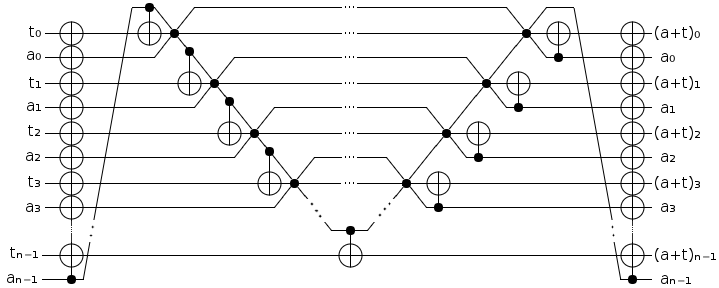
\includegraphics[totalheight=3cm]{inline-adder.png}
  \caption{\em Adder using no ancilla and $\Theta(N)$ CNOTs and CSWAPs. Based on [van2004].}
  \label{fig:inlineadder}
\end{figure}

To perform subtraction instead of addition: run the circuit in reverse, temporarily invert the target register by bordering the circuit with NOT gates on the target, or invert the CSWAP controls.

\section{$O(N)$ incrementer}

Note that a register can be incremented by subtracting both $x$ and $\neg x = -x-1$ from it for any $x$.
When $N$ dirty ancilla are available, this can be done directly as shown in figure \ref{fig:double-sub-increment}.

\begin{figure}
  \centering
  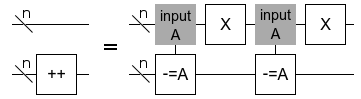
\includegraphics[totalheight=2cm]{double-sub-increment.png}
  \caption{\em Subtracting $x$ and $-x-1$ from a register increments it. Requires $O(N)$ depth, size, and $N$ dirty ancilla.}
  \label{fig:double-sub-increment}
\end{figure}

An increment gate can be decomposed into halves where the top half is incremented only if all of the bottom bits are on, and then the bottom half is incremented.
By borrowing the top half, the bottom half can be incremented with the double-subtraction trick.
But the trick doesn't work on the top half, because the top half can't be borrowed when being controlled by it.

A workaround for this is to change the second subtraction to an addition, and to conditionally toggle the target bits instead of the input bits.
When the condition isn't satisfied, the addition and subtraction cancel each other.
When the condition is satisfied, the addition inverts into a second subtraction and the input is subtracted from the target twice.
However, because we are conditioning on the input bits all being on, the input must be -1 and the target must have been incremented by 2.
To halve the +2 into a +1, left-shift the target and use a dirty bit as its LSB.

\begin{figure}
  \centering
  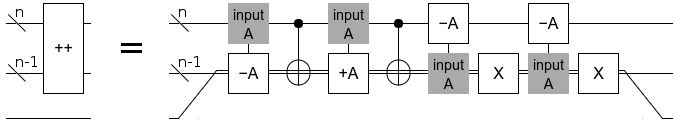
\includegraphics[totalheight=1.5cm]{compact-increment.png}
  \caption{\em Odd-sized $\Theta(N)$ increment with 1 dirty ancilla.}
  \label{fig:compact-increment}
\end{figure}

The described incrementer construction is shown in figure \ref{fig:compact-increment}.
However, because the adder/subtracter construction requires the target and source registers to be the same size, this incrementer construction only works on odd-sized registers.
For even-sized registers, another minor variation on the conditionally-invert-addition-into-subtraction-with-logical-negation technique is used.
The construction is shown in \ref{fig:compact-increment-even}.
Note that it is easily modified to perform efficient increments with arbitrarily many controls.

\begin{figure}
  \centering
  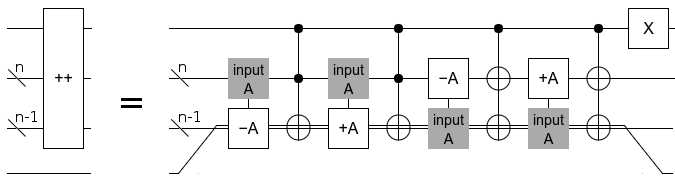
\includegraphics[totalheight=2cm]{compact-increment-even.png}
  \caption{\em Even-sized $\Theta(N)$ increment with 1 dirty ancilla.}
  \label{fig:compact-increment-even}
\end{figure}

As with addition and subtraction, you can turn an increment into a decrement either by reversing the gate order, by bordering the circuit with NOT gates, or by inverting all of the controls.

Our incrementer is classically optimal in asymptotic size and number of ancilla, but not depth.
The size is asymptotically optimal because any incrementer must touch all $n$ bits.
The number of ancilla is classically optimal, assuming we want to reduce to a fixed-size gate set, because the parity of the permutation performed by an increment operation is odd but the parity of the permutation performed by a classical gate that doesn't cover the entire circuit is even.
Therefore, without a dirty bit to use as workspace, no classical circuit can perform an increment gate.
Quantumly, the parity barrier can be bypassed by using partial rotations (see figure \ref{fig:bootstrap-ancilla}).

\begin{figure}
  \centering
  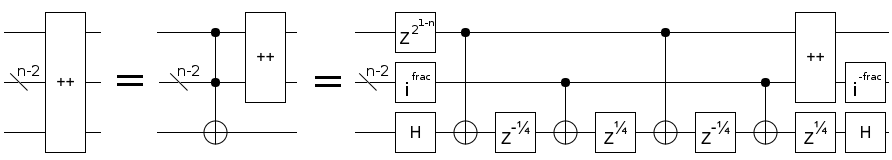
\includegraphics[totalheight=1.3cm]{ancilla-bootstrap.png}
  \caption{\em Bootstrapping dirty ancilla out of an increment gate using quantum operations.}
  \label{fig:bootstrap-ancilla}
\end{figure}

\section{$O(N \lg N)$ constant $\text{PivotFlip}$}

A pivot-flip operation reverses the order of states less than or equal to a given pivot value.
For example, a pivot-flip with the pivot equal to 3 would swap $|0\rangle$ and $|3\rangle$, swap $|1\rangle$ and $|2\rangle$, and leave all other states untouched.
We will use pivot-flips later, when implementing modular addition.

For concreteness, the exact permutation of a pivot-flip is:

$$\text{PivotFlip}_k = \sum_{i=0}^k |k-i\rangle \langle i| + \sum_{i=k+1}^{N-1} |i\rangle \langle i|$$

To perform a pivot-flip efficiently, we use the fact that $x \rightarrow \lnot(x - a)$ nearly does what is required.
However, instead of doing nothing to the elements past the pivot, it also flips those elements as shown in figure \ref{fig:double-flip}.

\begin{figure}
  \centering
  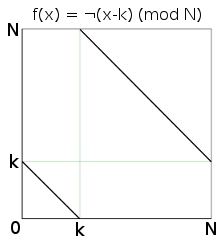
\includegraphics[totalheight=7cm]{double-flip.png}
  \caption{\em Subtraction followed by logical negation performs a flip both above and below the pivot.}
  \label{fig:double-flip}
\end{figure}

Note that $x \rightarrow \lnot(x - a)$ is its own inverse and maintains the invariant that a given value will cause an underflow when subtracting $a$.
So, by applying the operation twice, controlled by a dirty bit that is toggled by the underflow signal, the desired effect is achieved.
The part of the range below the pivot does trigger the underflow, so only one of the controlled flips happens.
The part of the range above the pivot does not cause an underflow, and so flips no times or two times, undoing itself.

The resulting pivot-flip circuit is shown in figure \ref{fig:const-pivot-flip}.

\begin{figure}
  \centering
  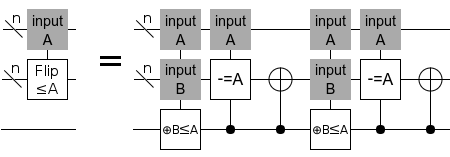
\includegraphics[totalheight=2cm]{pivot-flip.png}
  \caption{\em Pivot flip circuit.
  Note that the top wire bundle is a compile-time constant.
  The underflow toggle is done with an $n+1$-bit subtraction then an $n$-bit addition.
  [[[Requires an extra dirty bit for the n+1-bit subtraction?]]]
  The controlled subtractions are done by controlling every generated operation.}
  \label{fig:const-pivot-flip}
\end{figure}

Because the pivot is a compile-time constant, and so there is no source register workspace, the inline adder construction can't be used.
Instead, we use the constant-adder from [haner2016].
That adder requires $O(N)$ depth and $O(N \lg N)$ size, and therefore so does the constant-pivot-flip circuit.

\section{$O(N \lg N)$ Modular Constant-Adder}

A modular addition is three pivot flips.
To add $a$ modulo $n$, perform a pivot-flip at $n-a$, a pivot-flip at $n$, and then a pivot-flip at $a$.

[[[diagram]]]

Because the modular addition does a constant number of pivot-flips, its resource usage is identical: one [[[two?]]] dirty bits, $O(N)$ depth, and $O(N \lg N)$ size.

\section{$O(N)$ $\text{PivotFlip}$}

For completeness, we also discuss how to do a pivot-flip when the pivot is stored in a register instead of a compile-time constant.
The original construction doesn't work in this case because it uses an extra bit in the source register.

To work around the problem we propagate the increment into the operations on the target.
[[[But the addition sizes don't match up?]]]

[[[Maybe just ignore the increment size problem, then fixup with a conditioned all-flip?]]]

Note that, when storing in a register, we offset the pivot $k$ by one.
This is to avoid the redundancy $\text{PivotFlip}_0 = \text{PivotFlip}_1 = I$ and to move the flip-all operation $\text{PivotFlip}_{N}$ into range.
Concretely, we want to perform this permutation:

$$\text{RegisterPivotFlip} = \sum_{k=0}^{N-1} |k\rangle \langle k| \otimes \text{PivotFlip}_{k+1}$$

Basically we do this by just inlining the increments and decrements into the addition operations or by using that other thing I tried.

\section{$\Theta(N)$ Modular Addition}

Same high-level construction as the constant modular adder.
Do three pivot flips, but register-based instead of constant-based.
This reduces the size cost from $O(N \lg N)$ to $O(N)$.

\section{Applications}

Shor's algorithm in $2n+1$ qubits.





References:

haner2016 https://arxiv.org/abs/1611.07995
Factoring using 2n+2 qubits with Toffoli based modular multiplication
Thomas Häner, Martin Roetteler, Krysta M. Svore

van2004
Optimal Design of A Reversible Full Adder
YVAN VAN RENTERGEM AND ALEXIS DE VOS
2004

\end{document}
